\documentclass[fleqn,10pt]{SelfArx}
%----------------------------------------------------------------------------------------
%	Packages and definitions
%----------------------------------------------------------------------------------------

\usepackage{listings}
\usepackage{listings}
\usepackage{xcolor}
\definecolor{verylightgrey}{rgb}{0.97,0.97,0.97} % f7f7f7



\lstloadlanguages{sh,bash,HTML,python}

% general format
\lstset{
  captionpos=b,
  frame=single,frameround=tttt,
  framerule=0pt,
  backgroundcolor=\color{verylightgrey},
  xleftmargin=0.5cm,
  xrightmargin=0.5cm,
  showstringspaces=false,
  numbers=left, numberstyle=\tiny, stepnumber=1, numbersep=5pt,
  basicstyle=\scriptsize,
  breaklines=true,
  tabsize=2,
  float=ht!
}

\lstdefinelanguage{console}{
  morekeywords={},
  otherkeywords={warumgehtdasnicht>,\$}
}

\newcommand{\lstsetpython}
{ \vspace{\lstspace}
  \lstset{language=Python,
	 stringstyle=\color{blue},	
         moredelim=*[s][\color{darkviolet}]{$}{=}{$$$}, % option is makes delimiters invisible
	 moredelim=[s][\color{black}]{\"}{\"},
 }
}

\newcommand{\lstsetautoit}
{ \vspace{\lstspace}
  \lstset{%language=PHP,
	 stringstyle=\color{blue},	
         moredelim=*[s][\color{darkviolet}]{$}{=}{$$$}, % option 'is' makes delimiters invisible
	 moredelim=[s][\color{black}]{\"}{\"},
	 morecomment=[l]{;},
	 moredelim=[l][\color{blue}]{$$$}
% 	 moredelim=[l][\color{red}]{=},
% 	 moredelim=[l][\color{green}]{&}
 }
}

 % \lstinline$var i:integer;$ % for inline code snippets
 % \lstinputlisting{file.txt}

\newcommand{\lstsetconsole}
{ \vspace{\lstspace}
  \lstset{language=sh,
        lineskip=-2pt,
        language=console,
        commentstyle=\textit,
        keywordstyle=\bfseries,
        stringstyle=\ttfamily,
        showstringspaces=false,
	moredelim=[l][\color{black}\tbf]{\#}
  }
}


\newcommand{\lstsetjava}{
 \lstset{language=Java,
        commentstyle=\textit,
        keywordstyle=\bfseries,
        stringstyle=\ttfamily,
        showstringspaces=false,
        literate=
        %linewidth=\textwidth,captionpos=b
        %numbers=left, stepnumber=5, numbersep=10pt
 }
}


\newcommand{\lstsethtml}{
 \lstset{language=HTML,
        commentstyle=\textit,
        keywordstyle=\bfseries,
        stringstyle=\ttfamily,
        showstringspaces=false,
        %%linewidth=\textwidth,captionpos=b
        %numbers=left, stepnumber=5, numbersep=10pt
 }
}

\newcommand{\lstsetphp}{
 \lstset{language=PHP,
        breaklines=true,
        commentstyle=\textit,
        keywordstyle=\bfseries,
        basicstyle=\ttfamily,
        stringstyle=\ttfamily,
        showstringspaces=false,
        frame=single,
        tabsize=2
        %%linewidth=\textwidth,captionpos=b
        %numbers=left, stepnumber=5, numbersep=10pt
 }
} 

\lstnewenvironment{code}
    {\lstset{}%
      \csname lst@SetFirstLabel\endcsname}
    {\csname lst@SaveFirstLabel\endcsname}
\newcommand{\lstsethaskell}{
    \lstset{
      language=Haskell,
      commentstyle=\textit,
      keywordstyle=\bfseries,
      basicstyle=\ttfamily,
      stringstyle=\ttfamily,
      showstringspaces=false,
      frame=single,
      flexiblecolumns=false,
      basewidth={0.5em,0.45em},
      literate={+}{{$+$}}1 {/}{{$/$}}1 {*}{{$*$}}1 {=}{{$=$}}1
               {==}{{$==$}}2 %{!=}{{$\not\equiv$}}2
               {>}{{$>$}}1 {<}{{$<$}}1 {\\}{{$\lambda$}}1
               {\\\\}{{\char`\\\char`\\}}1
               {->}{{$\rightarrow$} }2 {>=}{{$\geq$}}2 {<-}{{$\leftarrow$}}2
               {<=}{{$\leq$}}2 {=>}{{$\Rightarrow$} }2
               {\ .}{{$\circ$}}2 {\ .\ }{{$\circ$}}2 {(.)}{({$\circ$})}2
               {>>}{{>>}}2 {>>=}{{>>=}}2
               {|}{{$\mid$}}1
    }
}

\lstdefinelanguage{JavaScript}{
  keywords={typeof, new, true, false, catch,%
    function, return, null, catch, switch, var,%
    if, in, while, do, else, case, break},
  ndkeywords={class, export, boolean, throw, implements, import, this},
  sensitive=false,
  comment=[l]{//},
  morecomment=[s]{/*}{*/},
  morestring=[b]',
  morestring=[b]"
}

\newcommand{\lstsetjavascript}{
  \lstset{
  language=JavaScript,
  breaklines=true,
  commentstyle=\textit,
  basicstyle=\ttfamily,
  keywordstyle=\bfseries,
  stringstyle=\ttfamily,
  showstringspaces=false,
  frame=single,
  tabsize=2
  }
}
\newcommand{\lstsetxml}{
 \lstset{language=XML,
        breaklines=true,
        commentstyle=\sffamily,
        keywordstyle=\bfseries,
        basicstyle=\sffamily,
        showstringspaces=false,
        stringstyle=\ttfamily,
        frame=single,
        tabsize=2,
        literate=
        %linewidth=\textwidth,captionpos=b
        %numbers=left, stepnumber=5, numbersep=10pt
 }
}
\lstdefinelanguage{CSharp}{
 morekeywords = {abstract,event,new,struct,as,explicit,%
    null,switch,base,extern,object,this,bool,false,%
    operator,throw,break,finally,out,true,byte,fixed,%
    override,try,case,float,params,typeof,catch,for,%
    private,uint,char,foreach,protected,ulong,checked,%
    goto,public,unchecked,class,if,readonly,unsafe,%
    const,implicit,ref,ushort,continue,in,return,using,%
    decimal,int,sbyte,virtual,default,interface,sealed,%
    volatile,delegate,internal,short,void,do,is,sizeof,%
    while,double,lock,stackalloc,else,long,static,%
    enum,namespace,string,partial},
  morecomment = [l]{//},
  morecomment = [l]{///},
  morecomment = [s]{/*}{*/},
  morestring=[b]",
  sensitive = true
}
\newcommand{\lstsetcsharp}{
 \lstset{language=csharp,
        breaklines=true,
        commentstyle=\sffamily,
        basicstyle=\sffamily,
        keywordstyle=\bfseries,
        stringstyle=\ttfamily,
        showstringspaces=false,
        frame=single,
        tabsize=2
        %%linewidth=\textwidth,captionpos=b
        %numbers=left, stepnumber=5, numbersep=10pt
 }
}
\lstdefinelanguage{FSharp}{
  morekeywords={abstract,and,as,assert,base,begin,%
    class,default,delegate,do,done,downcast,downto,%
    elif,else,end,exception,extern,false,finally,for,fun,%
    function,if,in,inherit,inline,interface,internal,lazy,%
    let,match,member,module,mutable,namespace,%
    new,not,null,of,open,or,override,private,public,rec,%
    return,static,struct,then,to,true,try,type,upcast,use,%
    val,void,when,while,with,yield,asr,land,lor,lsl,lsr,lxor,%
    mod,sig,atomic,break,checked,component,const,%
    constraint,constructor,continue,eager,event,external,%
    fixed,functor,global,include,method,mixin,object,%
    parallel,process,protected,pure,sealed,tailcall,trait,virtual,volatile},
  sensitive=false,
  morecomment=[l][\color{greencomments}]{///},
  morecomment=[l][\color{greencomments}]{//},
  morecomment=[s][\color{greencomments}]{{(*}{*)}},
  morestring=[b]"
}
\newcommand{\lstsetfsharp}{
 \lstset{language=fsharp,
        breaklines=true,
        commentstyle=\sffamily,
        basicstyle=\sffamily,
        keywordstyle=\bfseries,
        stringstyle=\ttfamily,
        showstringspaces=false,
        frame=single,
        tabsize=2
        %%linewidth=\textwidth,captionpos=b
        %numbers=left, stepnumber=5, numbersep=10pt
 }
}
\usepackage{subfigure}
\usepackage{indentfirst}
\usepackage{apacite}

%----------------------------------------------------------------------------------------
%	COLUMNS
%----------------------------------------------------------------------------------------

%\setlength{\columnsep}{0.55cm} % Distance between the two columns of text
\setlength{\fboxrule}{0.75pt} % Width of the border around the abstract

%----------------------------------------------------------------------------------------
%	COLORS
%----------------------------------------------------------------------------------------
\definecolor{color1}{gray}{0.30} % Color Ligth Gray 
%\definecolor{color1}{RGB}{0,0,90} % Color of the article title and sections
\definecolor{color2}{gray}{0.10} % Color Ligth Gray 
%\definecolor{color2}{RGB}{0,20,20} % Color of the boxes behind the abstract and headings

%----------------------------------------------------------------------------------------
%	HYPERLINKS
%----------------------------------------------------------------------------------------

\usepackage{hyperref} % Required for hyperlinks
\hypersetup{hidelinks,colorlinks,breaklinks=true,urlcolor=color2,citecolor=color1,linkcolor=color1,bookmarksopen=false,pdftitle={Title},pdfauthor={Author}}



%----------------------------------------------------------------------------------------
%	ARTICLE INFORMATION
%----------------------------------------------------------------------------------------

\ArticleInfo{Mayo 2015}%Vol. XXI, No. 1, 1-5, 2013} % Journal information
\Archive{} % Additional notes (e.g. copyright, DOI, review/research article)

\PaperTitle{Trabajo Final de Práctica} % Article title
\SubTitle{Seminario OS14 - Pattern Recognition}

\Authors{
Angel Cancio \textsuperscript{1*},
}% Authors

\affiliation{\textsuperscript{1}\textit{ITeDA, Mendoza, Argentina}}
\affiliation{*\textbf{Contacto}: angel.cancio@gmail.com} % Corresponding author

\Keywords{} % Keywords - if you don't want any simply remove all the text between the curly brackets
\newcommand{\keywordname}{Palabras Claves} % Defines the keywords heading name

%----------------------------------------------------------------------------------------
%	ABSTRACT
%----------------------------------------------------------------------------------------

\Abstract{Con este trabajo práctico se intenta estudiar el desempeño de distintas familias de clasificadores en función de la dimensión del espacio de características $\chi$ y el tamaño $n$ del conjunto $An={(x_1 , y_1 ), . . . , (x_n , y_n )}$ de datos de entrenamiento disponible para estimar la regla de decisión.}

%----------------------------------------------------------------------------------------

\begin{document}

\flushbottom % Makes all text pages the same height

\renewcommand{\abstractname}{Resumen}
\maketitle % Print the title and abstract box

\renewcommand{\contentsname}{Indice}
\tableofcontents % Print the contents section

\thispagestyle{empty} % Removes page numbering from the first page

%----------------------------------------------------------------------------------------
%	ARTICLE CONTENTS
%----------------------------------------------------------------------------------------


\section*{Actividades previas} % 
En función de lo trabajado en clases, para desarrollar la actividad propuesta será necesario
haber completado y así disponer de códigos computacionales que implementen los siguientes
procedimientos:
\begin{itemize}
\item Clasificador de $K$ vecinos más cercanos, con posibilidad de variar el valor de $K$.
\item Clasificador por estimación de densidades de tipo Parzen, con posibilidad de variar el parámetro característico del kernel usado.
\item Clasificador suponiendo que las distribuciones de probabilidad de ambas clases son Gaussianas (discriminante lineal y cuadrático)
\item Clasificador por máquinas de vector soporte (SVM), con posibilidad de variar el parámetro característico del kernel usado y el valor de C.
\item Procedimiento de extracción de características usando KPCA.
\item Procedimiento general de validación cruzada para estimar errores de predicción.
\end{itemize}

\section*{Actividades a desarrollar} % 
El archivo \texttt{datosOS14.mat} contiene datos correspondientes a un problema de clasificación de vocales. Se han extraído solamente dos vocales, para trabajar con clasificación binaria.
\begin{enumerate}
\item Extraiga al azar un subconjunto de entrenamiento de $n_{train} = 80$ datos en total. Reserve el resto de las muestras para estimar el error de predicción. Utilice el conjunto de entrenamiento obtenido para entrenar un clasificador automático de las vocales del problema, usando las siguientes estrategias:
\begin{itemize}
\item k-vecinos más cercanos
\item estimación de densidades tipo Parzen
\item discriminante lineal y cuadrático
\item SVC basado en kernels
\item $KPCA+k-$vecinos más cercanos
\item $KPCA+$estimación de densidades tipo Parzen
\end{itemize}

\item Repita el procedimiento anterior 10 veces. Reporte el error de predicción promedio para
cada tipo de clasificador, usando los resultados de las 10 repeticiones. Reporte también el desvío estándar de los resultados. ¿Encontró mucha variabilidad entre las distintas repeticiones en los valores de los parámetros óptimos de los clasificadores (cantidad de vecinos, ancho de banda de kernels, etc)? Comente.

\item Repita los puntos 1) y 2) para $n_{train} = 120$, $150$, $n$, con $n$ la cantidad total de datos. Extraiga conclusiones.

\item Escriba un reporte de no más de dos páginas de extensión con sus conclusiones. Adjunte los códigos de cómputo utilizados.
\end{enumerate}

\section*{Desarrollo}

En el gráfico siguiente se puede observar la estimacion del error cometido durante las 10 repeticiones para cada clasificador, antes y despues de utilizar KPCA sobre los datos.

\begin{center}
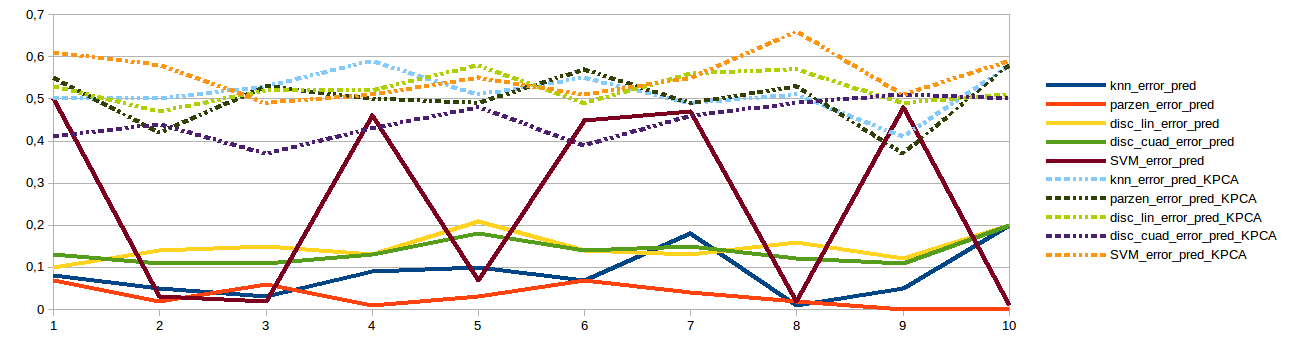
\includegraphics[scale=0.35]{fig/1.png} 
\end{center}

En el gráfico siguiente se puede observar la variacion del error error cometido durante la validacion cruzada para las 10 repeticiones para cada clasificador, antes y despues de utilizar KPCA sobre los datos.

\begin{center}
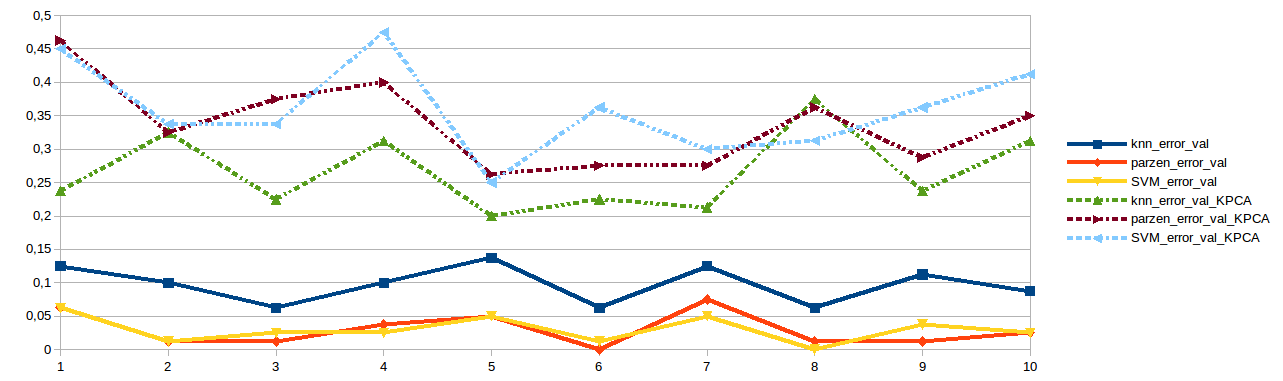
\includegraphics[scale=0.35]{fig/2.png} 
\end{center}

El siguiente gráfico muestra como mejora la clasificación de los datos conforme se aumenta el tamaño de la muestra. 

También se observa que KNN con K=1 es invariante respecto al tamaño de la muestra, pero en terminos de rendimiento computacional KNN se encarece al aumentar la dimensionalidad.

El clasificador de ventana de parzen se encuetra fectado por la independencia de las dos clases.  

\begin{center}
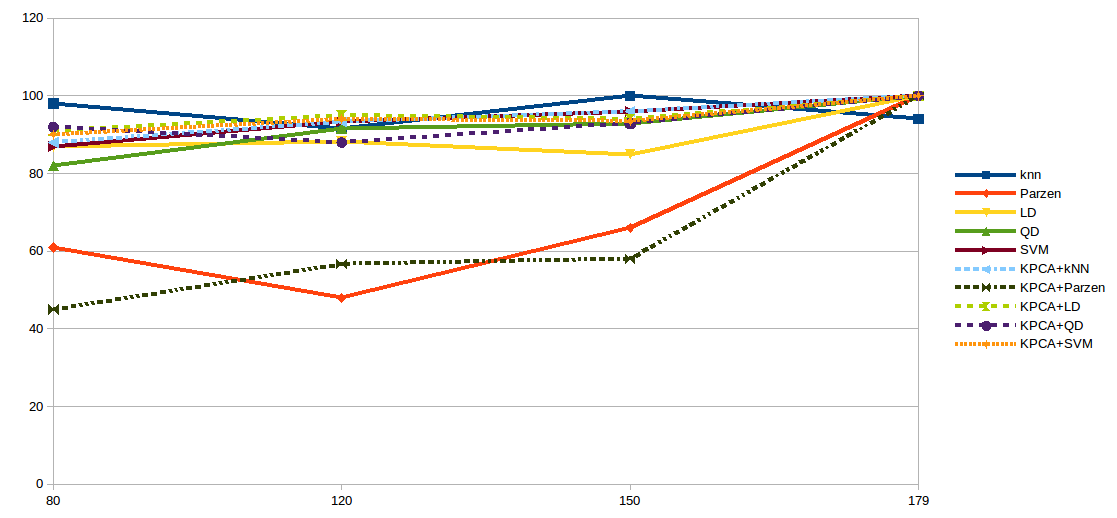
\includegraphics[scale=0.35]{fig/3.png} 
\end{center}

\section*{Concluciones}

Despues de haber probado los distintos clasificadores (kNN, Parzen, Discriminador Lineal, Discriminador Cuadratico) sin aplicar la transformacion por analisis de componente principales y luego aplicando la transformacion utilizando analisis de componente principales (PCA y KPCA), y se llega a la conclucion de que es importante tener en cuenta tres puntos: 1) Es necesario realizar una normalizacion y estandarización de los datos antes de realizar la clacificación (pre\-procesamiento), 2) Es muy importante realizar una validación cruzada para ajustar los parámetros del modelo del  clasificador ya que hay una importante variación según el set de entrenamiento utilizado. 3) Y por último el uso de transformaciones de espacio como PCA, KPCA o inclusive los discriminadores de Fisher LDA y QDA permiten reducir la dimencionalidad de los datos y eventualmente encontrar una proyección óptima para poder visualizarlos.

Con las transformaciones espaciales: se provee conjunto relevante de características al clasificador (mejora de desempeño particularmente en clasificadores simples). Se reduce la redundancia y se recuperan las características latentes más significativas de cada característica. Se genera mayor comprensión del proceso de generación de los datos.

%
%\section*{Introducción} % The \section*{} command stops section numbering
%\addcontentsline{toc}{section}{Introducción} % Adds this section to the table of contents
%
%%------------------------------------------------
%
%\section*{Marco Teórico} % The \section*{} command stops section numbering
%\addcontentsline{toc}{section}{Marco Teórico} % Adds this section to the table of contents
%
%\section*{Objetivos}
%\addcontentsline{toc}{section}{Objetivos}
%
%\section*{Métodos}
%\addcontentsline{toc}{section}{Métodos}
%
%\subsection*{Detalles}
%\addcontentsline{toc}{subsection}{Detalles}
%
%\section*{Resultados}
%\addcontentsline{toc}{section}{Resultados}
%
%\section*{Conclusiones} % The \section*{} command stops section numbering
%\addcontentsline{toc}{section}{Conclusiones} % Adds this section to the table of contents
%%----------------------------------------------------------------------------------------
%%	REFERENCE LIST
%%----------------------------------------------------------------------------------------
%\phantomsection
%\renewcommand{\refname}{Referencias} %% Para article
%%\renewcommand{\bibname}{Bibliografía} %% Para Book
%\bibliographystyle{apacite}	% or "siam", or "alpha", or "abbrv"
%
%\nocite{*}		% list all refs in database, cited or not.
%\bibliography{refereces.bib}		% bib database file refs.bib

%----------------------------------------------------------------------------------------

\pagebreak
\phantomsection
\section*{Apendice 1}

\begin{figure}[hbtp]
\caption{Proyeccion de datos originales usando los primeros dos features}
\centering
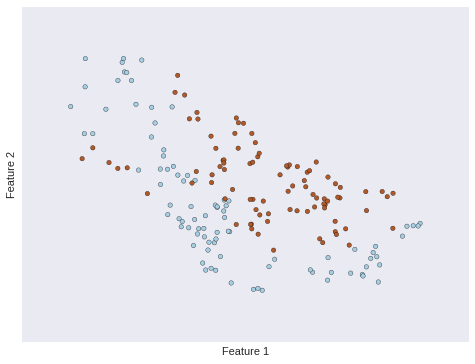
\includegraphics[scale=0.4]{fig/sinKPCA.png}
\end{figure}
\begin{figure}[hbtp]
\caption{Proyección despues de aplicar KPCA a los datos originales (primeros dos features). }
\centering
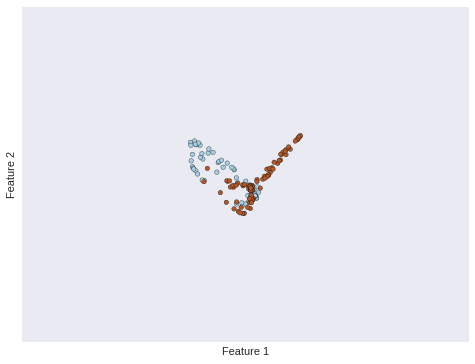
\includegraphics[scale=0.4]{fig/conKPCA.png}
\end{figure}

En la imagen se puede ver la clasificcacion usando Discriminante Lineal (izquierda) y Dirciminante Cuadrático (derecha) antes y despues de aplicar KPCA.


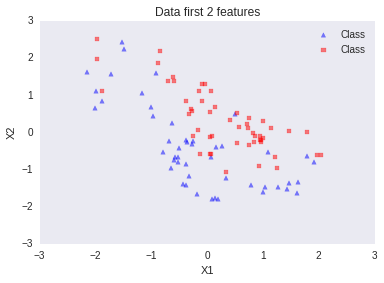
\includegraphics[scale=0.5]{fig/LD_pred.png}
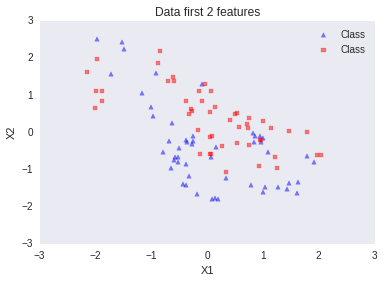
\includegraphics[scale=0.5]{fig/QD_Pred.png}

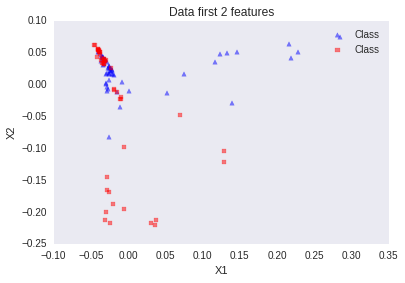
\includegraphics[scale=0.5]{fig/KPCA-LD_pred.png}
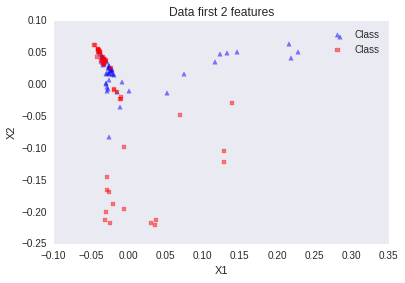
\includegraphics[scale=0.5]{fig/KPCA-QD_pred.png}

Por ultimo la representación de los datos en una matriz de confución muestra la superpocision de las distribuciones entre todas las caracteristicas de las N observaciones.

\centering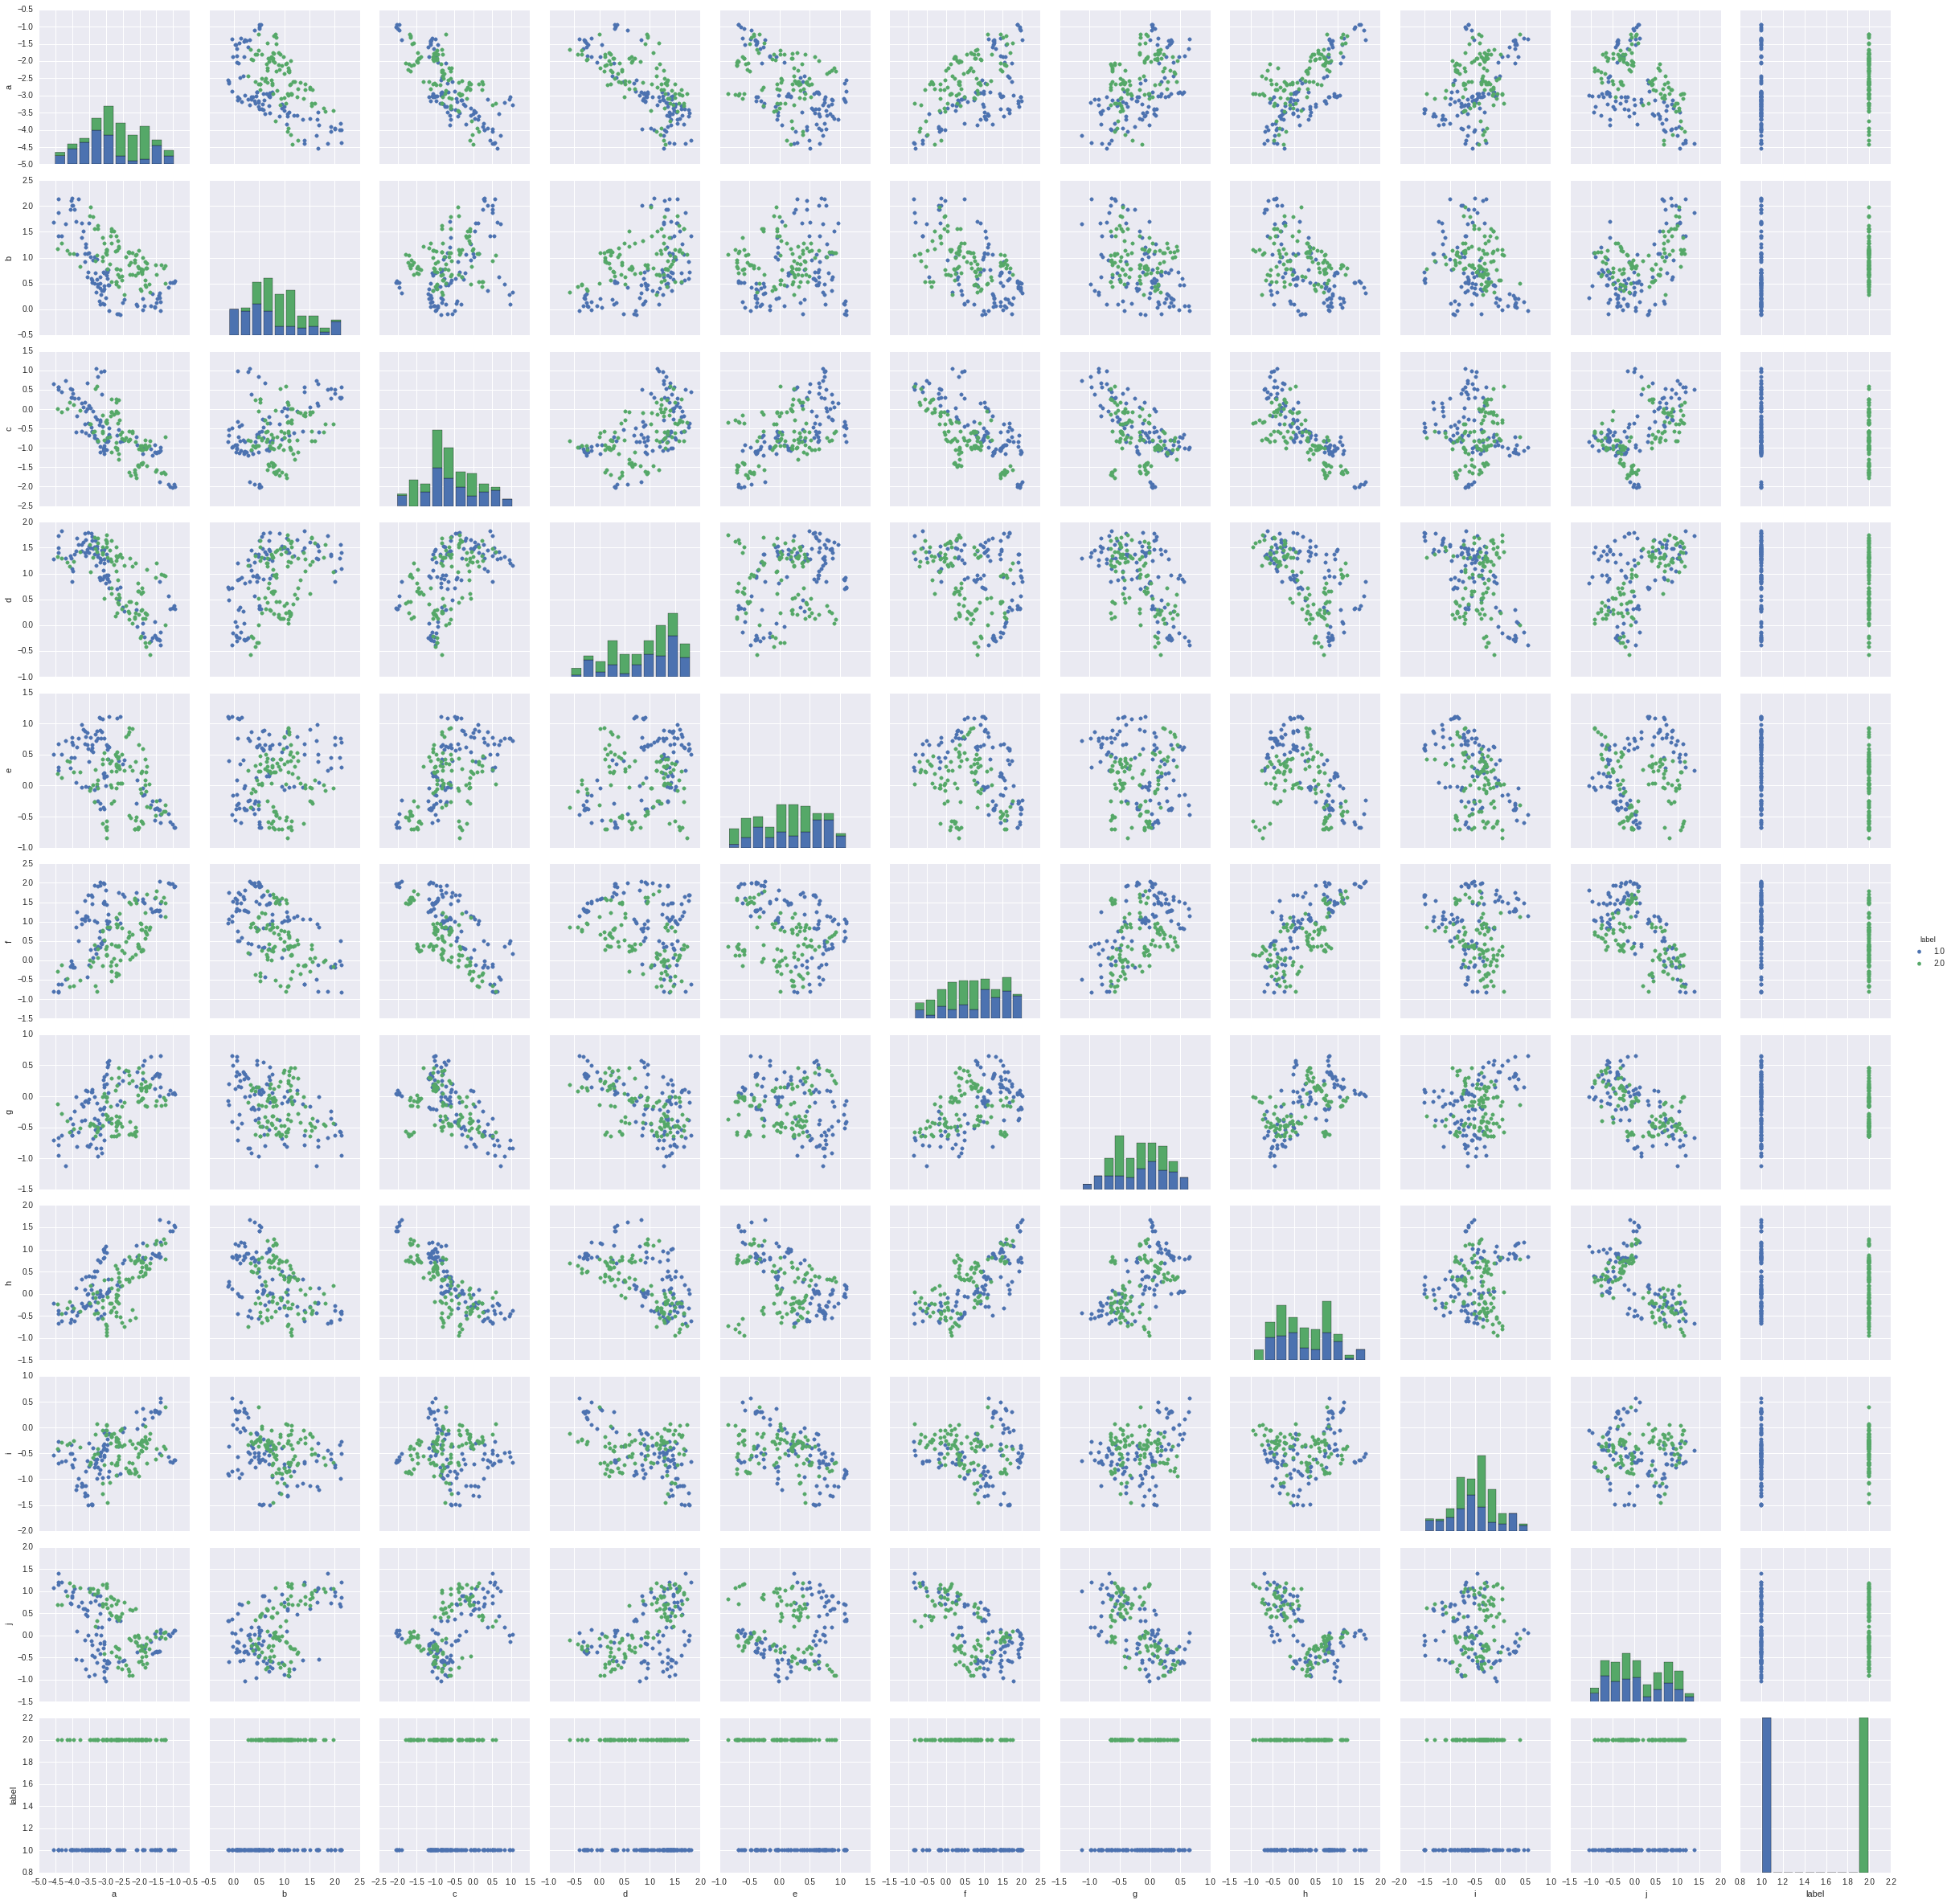
\includegraphics[scale=0.15]{fig/dataset.png} 

\end{document}